\documentclass[a4paper]{article}
\usepackage[margin=1.25in]{geometry}
\usepackage{amsmath}
\usepackage{ragged2e}
\usepackage[table,xcdraw]{xcolor}
\title{Low Frequency Impedances}
\date{February 27, 2018}
\author{Pablo Sevilla}
\usepackage{graphicx} 
\usepackage{float}
\usepackage{subcaption}



\begin{document}
  \pagenumbering{gobble}
  \maketitle
  \pagenumbering{arabic}
  
\begin{center}
  \section*{Abstract}
  \centering
  The output voltage of a given voltage source was calculated using a multi-meter. The internal resistance was also calculated by using a variable resistor connected in series. A different setup was later used to measure separately the impedance of three two-terminal black boxes with unknown components and configuration. The components were either a resistor, capacitor, inductor or a combination of two of these either in parallel or series. Using a DC current, and various AC frequencies, impedance behavior was compared to the common RLC models. Finally, a diode was examined by plotting a graph of current vs voltage to determine when the diode starts conducting. The first black box was found to contain a resistor and a capacitor in parallel. Another black box contained a single capacitor while the last black box contained RLC in series. The diode was found to allow current to flow in one direction only.
\end{center}
  
  \newpage
  
  \section{Introduction}
  \subsection{Output Impedance}
  Impedance refers to the measure of a circuit's struggle to undergo a flow of charge. When the current is independent of time, it is often referred as a direct current (DC), and its impedance is simply called resistance. A voltage source manufactured as $9V$, for example, will actually provide a voltage difference slightly lower than that. This is due to the physical limitations of the device, that force the existence of an impedance, or internal resistance $R_0$. According to Thevenin's theorem of linear circuit analysis, any two-terminal network of resistors and voltage sources is equivalent to a single resistor $R_0$ in series with a voltage source $V_0$. When the current is zero, the potential difference between the two terminals is equal to the output voltage $V_0$. 
  
  \begin{figure}[h]
\centering
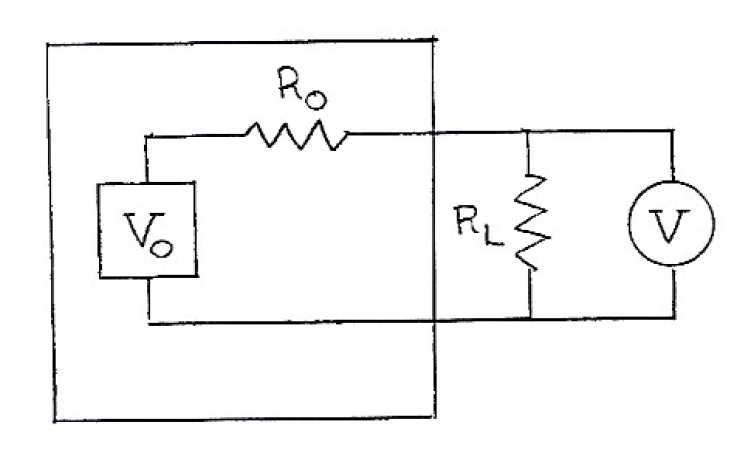
\includegraphics[width=0.5\textwidth]{voltagesource}
\caption{Circuit used to calculate internal resistance $R_0$ of a voltage source. An variable load resistor $R_L$ was tweaked and voltage behavior $V$ was observed. (Figure taken from Physics 133 lab manual at UC Santa Cruz)}
\end{figure}

When an extrinsic resistor $R_L$ is connected to the circuit (see figure above), a flow of charge $I$ will be induced in the circuit, dropping the voltage from $V_0$ to $V$ almost instantaneously. The relationship between these quantities is the following,

\begin{equation}
V=V_0-IR_0
\end{equation}

During this experiment, the true output voltage and internal resistance values for a given voltage source will be calculated. 

\subsection{Unidentified Linear Black Boxes}

In order to assess the contents and configuration of the black boxes, it is crucial that we generalize our concept of impedance to alternating currents (AC). An oscillating current as a function of time is often expressed as:

\begin{equation}
I(t)=I_0 cos(wt-\phi)
\end{equation}

where $I_0$ is the current at $t=0$, $w$ is the angular frequency and $\phi$ is the phase difference. When an RLC component is supplied with such alternating current, a time dependent potential difference between the two terminals of the device is created. Using $V_R=I(t)R$, $V_L=L\frac{dI(t)}{dt}$ and $V_C=\frac{1}{C}\int I(t)dt$, the respective voltages can be expressed as:
\clearpage
\begin{figure}[h]
\[ V_{resistor}=RI_ocos(wt-\phi)\] 
\[V_{inductor}=wLI_0cos(wt-\phi + \frac{\pi}{2})\]
\[V_{capacitor}=\frac{1}{wC}I_0cos(wt-\phi - \frac{\pi}{2})\]
\end{figure}

For the resistor case, the voltage phase difference is equal to the current's. Therefore, they are in phase. On the other hand, the inductor and capacitor do not share the same cosine argument, making the voltage lead or lag the current by a factor of $\frac{\pi}{2}$. This breaks down the linearity between $V$ and $I$.

By using complex variables to analyze these quantities, linearity can be imposed. Breaking down the current as real and imaginary components and using Euler's identity, we can obtain:
\begin{equation}
I(t)=I_r+jI_i=I_0(cos(wt-\phi)+jsin(wt-\phi)=I_oe^{jwt}
\end{equation}
where $j=\sqrt{-1}$. Using the same relationships as the ones used to derive RLC voltages, we can obtain a complex relationship between $V$ and $I$. 

\begin{figure}[h]
\[V_{inductor}=(jwL)I(t)\]
\[V_{capacitor}=(\frac{1}{jwC})I(t)\]
\end{figure}

We have now achieved linearity between these two quantities. The constant of proportionality is referred as the complex impedance, with symbol $Z$. The complex impedance for each device is:
\begin{figure}[h]
\[Z_R=R\]
\[Z_L=jwL\]
\[Z_C=\frac{1}{jwC}\]
\end{figure}

By using different combinations of resistors, inductors and capacitors, commonly referred as RLC circuits, particular impedance behaviors can be observed. It is important to understand that complex impedance adds linearly in series and reciprocally in parallel. A circuit will be constructed to observe the impedance of the black boxes as a function of frequency, $Z(w)$.

\subsection{Nonlinear Elements}

Diodes are two-terminal semiconductors that are designed to allow current to flow in only one direction. This is achieved thanks to the p-n junction installed inside the diode. When a voltage $V$ is supplied, it results in a that can be current expressed as:
\begin{equation}
I=I_S(e^{eV/kT}-1)
\end{equation}
where $I_S$ is the saturation current, $e$ is the elementary charge, $V$ is the applied voltage, $k$ is Boltmann's constant and $T$ is the temperature. 

A diode will be analyzed in this experiment to check that the relationship between current and voltage is not linear, but some curve.
\clearpage
\section{Procedure}
\subsection*{Apparatus}
\begin{itemize}
  \item \textbf{9V battery (x1)} - Two-terminal device that supplies a potential difference. Used to determine its internal resistance and experimental output voltage.
  \item \textbf{Diode (x1)} - Device that allows current to flow in one direction only. Used to check its non-linear proportionality between current and voltage.
  \item \textbf{Black Box (x3)} - Two-terminal devices with an unknown RLC configuration. Part of the aim of this investigation is to determine its components and configuration.
  \item \textbf{Multimeter (x1)} - Digital device able to measure voltage, current and resistance. It was used to calculate DC impedance of battery and the resistance of the black boxes. It was also used to check the precision of the variable resistor.
  \item \textbf{Variable Resistor (x1)} - A resistor with a adjustable resistances, ranging from $1\Omega$ to $4M\Omega$. It was used as the load resistor in the DC impedance circuit to control the independent variable. It was also used in the black box impedance-detecting circuit as means to keep voltages across the black box and the oscilloscope channels within a factor of 10 of each other.
  \item \textbf{Oscilloscope (x1)} - A digital device able to plot voltage information as a function of time. Cursor functions are available to compare two voltage channels. This device was used to calculate the amplitudes of the voltage oscillations and phase differences.
  \item \textbf{Function Generator (x1)} - A device that provides an alternating current in sinusoidal form. It has dials that can modify both its amplitude and frequency. It was used to vary the independent variable $w$ in the black box impedance configuration.
\end{itemize}
\subsection{Output Impedance}
The $9V$ battery was connected to the multimeter to measure its realistic voltage output. Subsequently a load resistor was attached in the following configuration:
\begin{figure}[h]
\centering
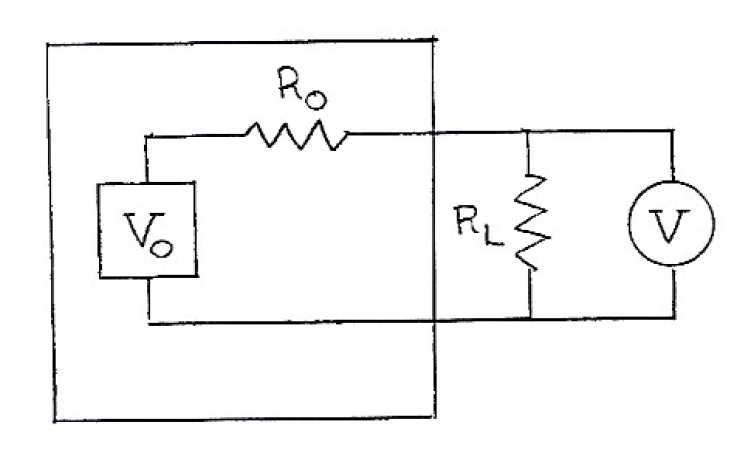
\includegraphics[width=0.5\textwidth]{voltagesource}
\end{figure}
Data was taken by changing the resistance of the internal resistor, with range of $500-3000\Omega$. The resulting current and voltage were reported with the multimeter. A plot of voltage vs. current was done, resulting in a linear relationship. The slope of such line was calculated to report the internal resistance of the battery, $R_0$. The graph was extrapolated to determine the $V(t=0)$ intercept. Such value corresponds to the experimental output voltage of the battery.

\subsection{Unknown Linear Black Boxes}
The aim of this experiment is to determine the components of the 3 black boxes. Firstly, the DC resistance of each black box was reported using the multimeter. This might provide useful preliminary information about the contents of the device, as capacitors have infinite resistance while inductors have very small resistance.

Subsequently, the following new circuit was assembled in order to measure the impedance under various frequencies:
 \begin{figure}[h]
\centering
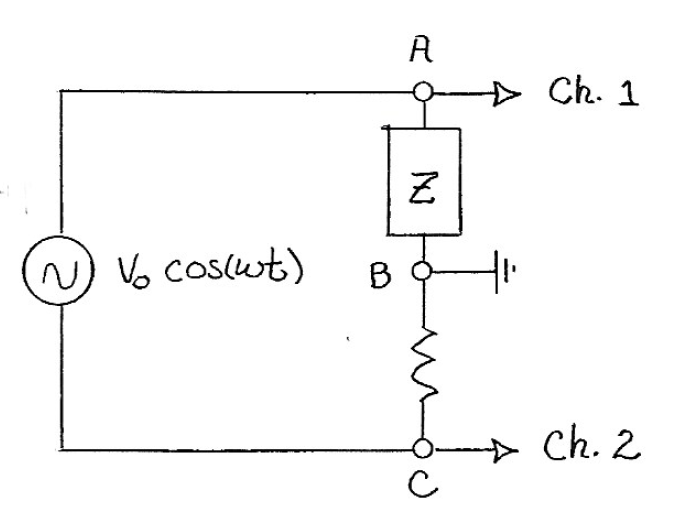
\includegraphics[width=0.5\textwidth]{zcircuit}
\caption{Circuit consisting of black boz $Z$, variable resistor, function generator and oscilloscope. Such configuration allowed to report the impedance under different frequencies. (Figure taken from Physics 133 lab manual at UC Santa Cruz)}
\end{figure}

The function generator, black box and variable resistor were connected in series, while the oscilloscope was connected in parallel to both the black box and the resistor separately. This resulted in two channels in the oscilloscope's display. Channel 1, connected to the black box, outputs voltage while Channel 2, connected to the resistor, outputs current, both as a function of time. The amplitudes of both channels were reported for around 25 data points, ranging from $1$ to 1x$10^{5}$ Hertz. At each data point, the phase difference between both channels was measured using the oscilloscope's cursor function. The variable resistor's resistance was tweaked multiple times for each black box in order to keep the voltages across the resistor and the black box within a factor of 10 of each other. 

The data obtained through this procedure allowed for calculations of the complex impedance $Z$ and also its magnitude, $|Z|$. These calculations provide the final clue for making an educated guess on the components of the unknown black box, as well as its configuration.

\subsection{Nonlinear Elements}

Using the same circuit configuration as in Figure 2, a diode was investigated qualitatively using the oscilloscope's XY function. This function plots a trace of the components behavior to flow of charge and potential difference. The current generates a vertical trace deflection on the display, while the voltage across the diode generates a horizontal trace deflection. This results in a well-defined trace on the display that provides an analog signature for the component.

The signature for the diode was recorded and later analyzed to check that it it indeed follows a non-linear relationship between voltage and current. A linear relationship would cause a signature shaped like a straight line with slope equal to the constant of proportionality. In addition, spike voltage of the diode will be observed.

\section{Data and Analysis}
\subsection{Output Impedance}
The output voltage for the battery was measured to be $8.37V$. The load resistor was connected to the voltage source and the voltage was measured with the multimeter. The resulting data is the following:
\clearpage
\begin{figure}[h]
\centering
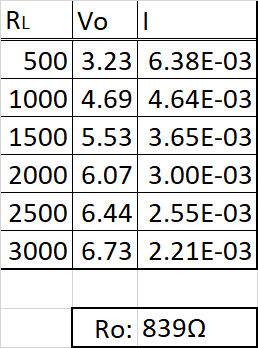
\includegraphics[width=0.25\textwidth]{batterydata}
\end{figure}
Using Ohm's Law, $V=IR$, the current that was going through the circuit for each load resistance was found. With this new information, a plot of voltage vs current was made and it was found that the data resembled a linear proportionality, therefore a linear regression was used. Such plot corresponds to the following equation:
\begin{equation*}
V=V_0-IR_0
\end{equation*}
\begin{figure}[h]
\centering
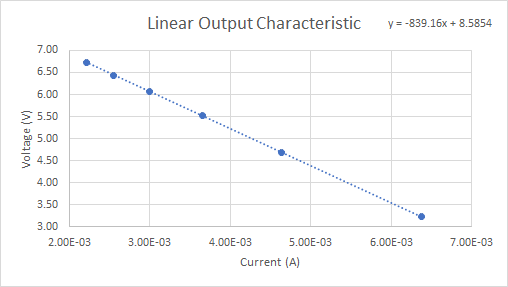
\includegraphics[width=1.0\textwidth]{batteryplot}
\end{figure}

The graph above shows a straight line with slope of $-R_0$ and y-intercept of $V_0$. It was found that the internal resistance was $839\Omega$ and the output voltage $V_0$ was $8.59V$. We can notice some inconsistencies with the previous measurement for the voltage of the battery, which was slightly lower. This might have been caused by the battery draining while being used and due to the internal resistance of the battery which lowers the output voltage.
\clearpage
\subsection{Unknown Linear Black Boxes}
\subsubsection{Box D}
Box D was connected to the circuit configuration as shown in Figure 2. Using the measurement tools on the oscilloscope, peak to peak voltage of Channel 1 and peak to peak voltage of Channel 2 was measured, along with the resistance of the load resistor, and the phase difference between the two wave forms. Using the cursor function, the phase difference was calculated by measuring the time of one full oscillation, dividing difference in time between two peaks of the two channels and multiplying the result by $360°$. The resulting value corresponds to the phase difference measured in degrees. The data obtained is shown in the following table:

\begin{figure}[h]
\centering
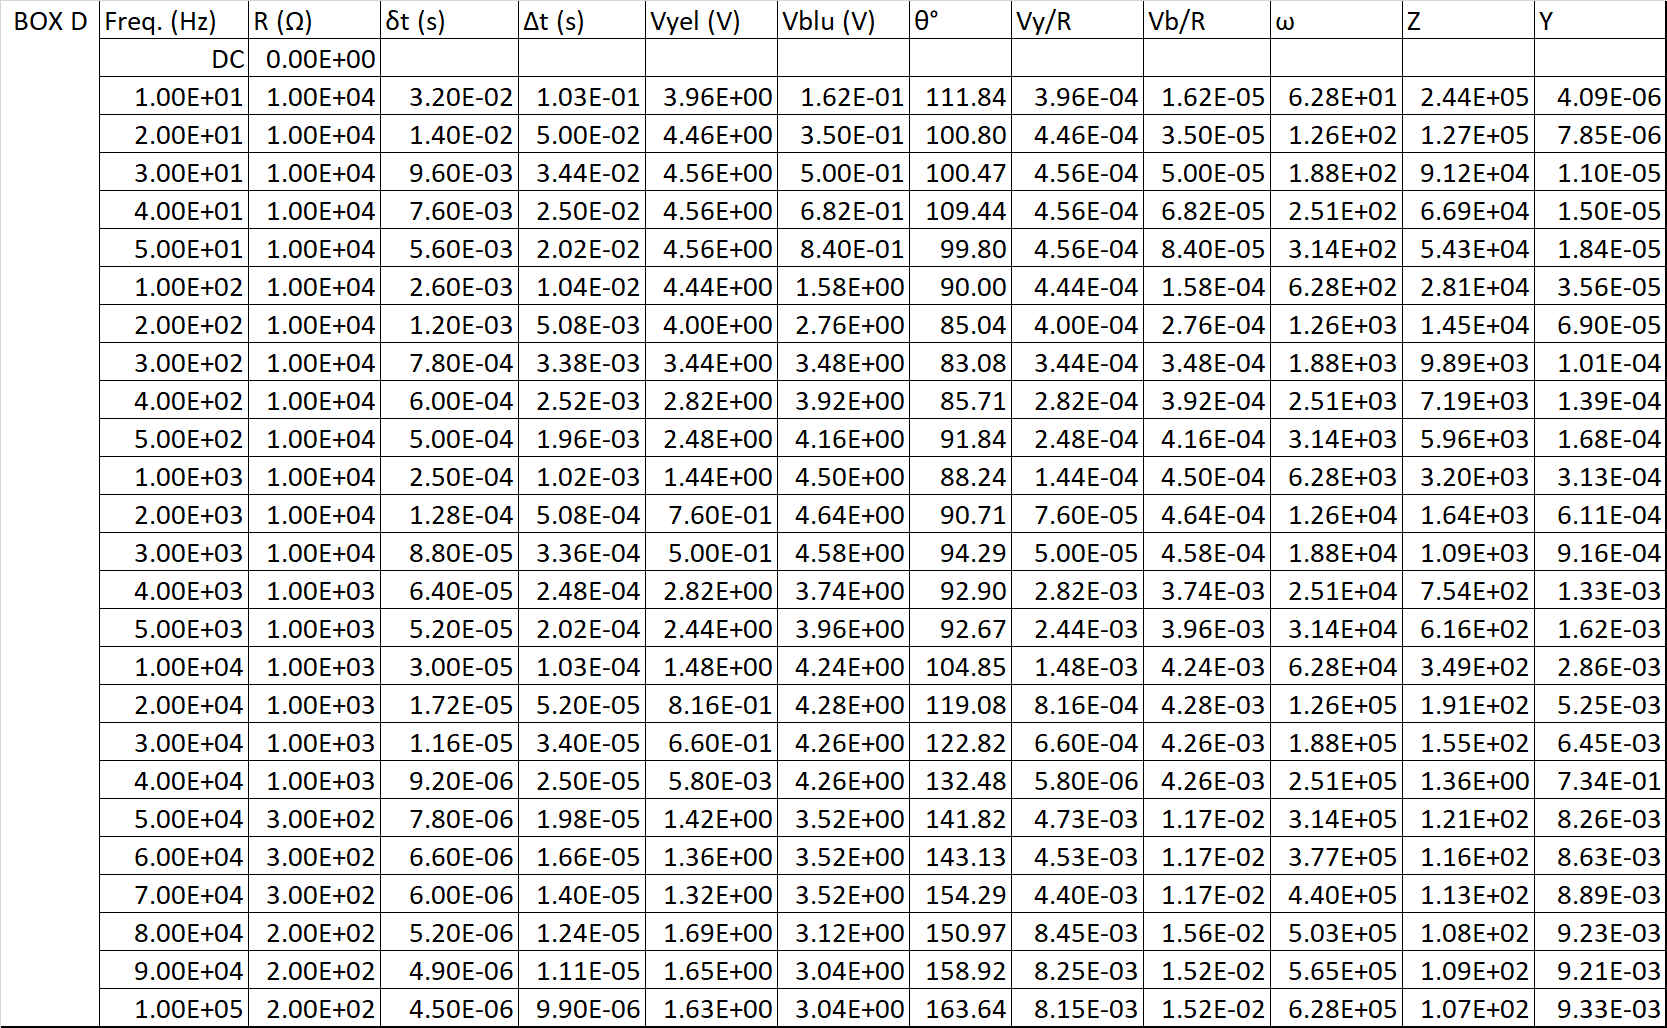
\includegraphics[width=1.0\textwidth]{boxd}
\end{figure}

The DC resistance of box D was measured using the multimeter and was found to be too high for the detector's sensitivity. This strongly suggests the existence of a capacitor in series. As the independent variable, in this case frequency, was increased it could be seen that the voltage lagged the current, as well as the voltage tending towards a minimum as the current increased. In addition, no resonance was detected, and this is a sign that indicates the lack of an inductor in Box D. With this quantitative and qualitative data, the following hypothesis for the contents and configuration of the black box was made:

\begin{figure}[h]
\centering
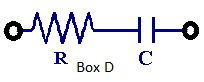
\includegraphics[width=0.85\textwidth]{boxdconfig}
\caption{Circuit configuration for a resistor and a capacitor in series.}
\end{figure}

\begin{figure}[h]
\centering
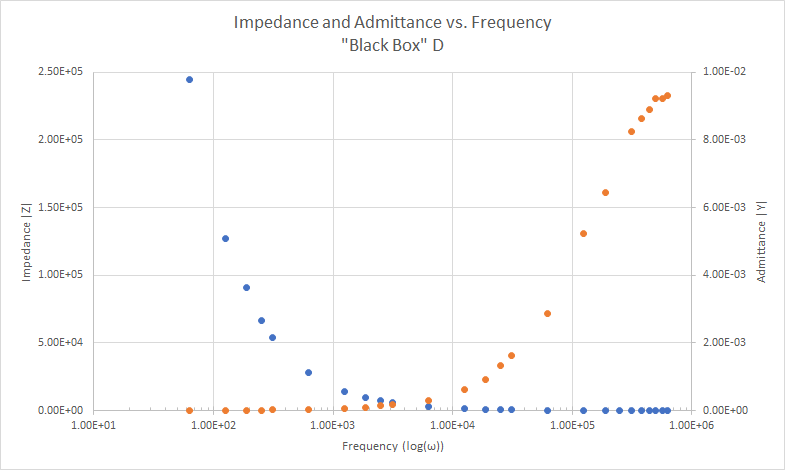
\includegraphics[width=0.85\textwidth]{boxdplot}
\caption{Graph of impedance vs. log of frequency for Box D. The admittance $|Y|=\frac{1}{|Z|}$ was plotted on top for visualization purposes and qualitative understanding. The impedance was measured using Equation (6), while the frequency values were calculated using the previous approach. }
\end{figure}

According to the theoretical impedance derived in Section 1.2, the complex impedance of this black box can be expressed as:
\begin{equation}
Z_{D} = Z_{resistor}+Z_{capacitor}=R+\frac{1}{jwC}
\end{equation}

In order to check for that this derived complex quantity is consistent with the data, the real magnitude of the complex impedance must be taken. This arises due to the fact that complex quantities cannot be observed experimentally, only real quantities. The magnitude of the complex impedance will be real. Squaring both sides and taking the square root of the argument:
\begin{equation}
|Z_{D}| = \sqrt{R+\frac{1}{jwC}}
\end{equation}

According to complex analysis, the phase of the circuit can be found theoretically by taking the tangent of the angle in the complex plane. This results in:
\begin{equation}
tan{\theta}=-\frac{1}{RwC}
\end{equation}

This is useful when calculating the actual values of the components. Using Kirchhoff's Laws, the capacitance of the circuit was found to be $C=3.3\times10^{-7}F$.  Using this information and the phase angle from the results table, the resistance of the hypothesized resistor can be found using Equation (7). This resistance was found to be $1329.7\Omega$. 

In order to experimentally check our results, a linear regression can be made that will provide parameters analogous to the resistance and capacitance of the black box. By plotting $\frac{1}{w^2}$vs.$|Z|^{2}$, a linear regression can be obtained with slope equal to $C^2$ and intercept on $\frac{1}{R^{2}}$. The resulting plot is the following:
\clearpage
\begin{figure}[h]
\centering
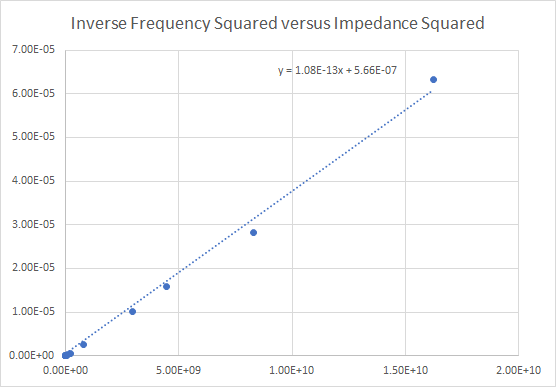
\includegraphics[width=0.85\textwidth]{boxdlinear}
\end{figure}
According to the parameters of the line of best fit, the capacitance was found to be $C=3.3\times10^{-7}F$ and the resistance $1329.7\Omega$. Thus the data recorded agrees with the hypothesis that Box D contains a resistor and a capacitor in series.
\clearpage
\subsection{Box A}
Using the same methods as for Box D, the following data was obtained:
\begin{figure}[h]
\centering
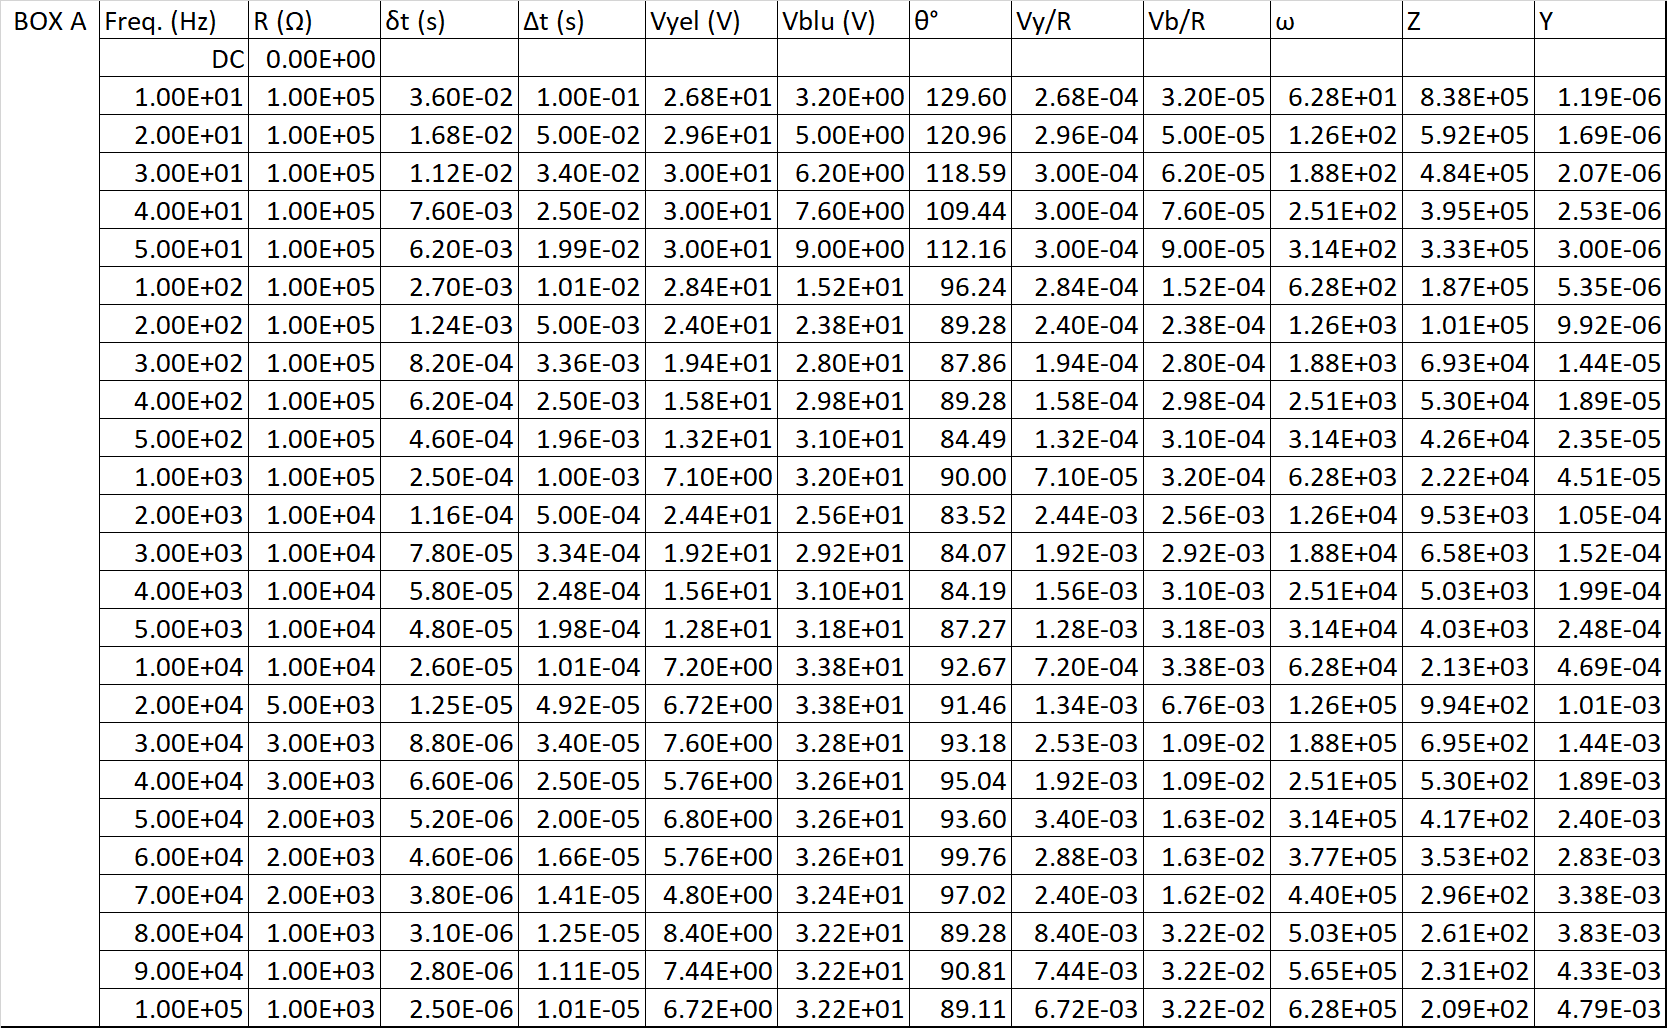
\includegraphics[width=1.0\textwidth]{boxa}
\end{figure}

The DC resistance of Box A was measured to be too large for the multimeter to handle, potentially infinite. This suggests the existence of a capacitor. This data shows a lack of correlation between impedance and frequency, implying the in-existence of an inductor. The question towards whether there is a resistor or not is puzzling. If there was one, it would have to be in series. This is due to the fact that resistance exponentially decayed as frequency was increased. Furthermore, a resistor and a capacitor in parallel would have not shown infinite DC resistance, therefore the parallel configuration can be discarded. The following plot of impedance vs. angular frequency was obtained:
\begin{figure}[h]
\centering
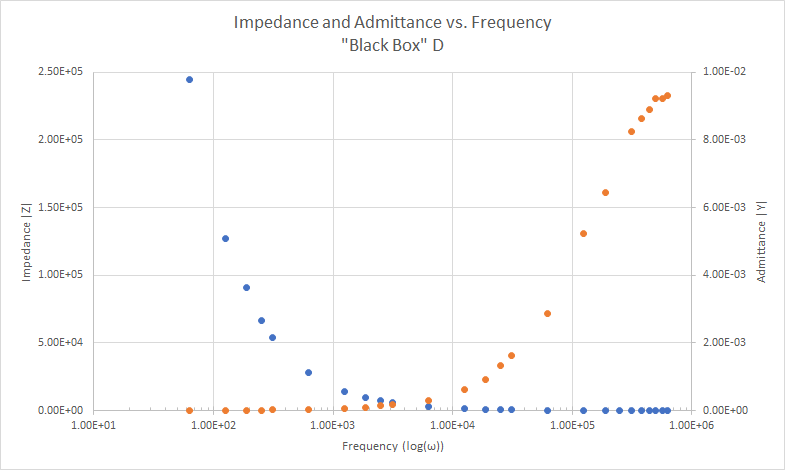
\includegraphics[width=0.71\textwidth]{boxdplot}
\caption{Graph of impedance vs. log of frequency for Box A. The admittance $|Y|=\frac{1}{|Z|}$ was plotted on top for visualization purposes and qualitative understanding. The impedance was measured using Equation (6), while the frequency values were calculated using the previous approach. }
\end{figure}

The plot obtained shows a pure exponential decay. This is indicative that the components must be either a single capacitor or a resistor and a capacitor. Due to the dependence of phase angle with frequency, it is likely that the box indeed has a resistor. Using Kirchhoff's Laws, the capacitance of the circuit was found to be $C=2.1\times10^{-7}F$.  Using this information and the phase angle from the results table, the resistance of the hypothesized resistor can be found using Equation (7). This resistance was found to be $2659.7\Omega$. 

\begin{figure}[h]
\centering
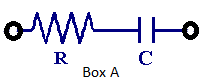
\includegraphics[width=0.85\textwidth]{boxaconfig}
\end{figure}

In order to assess the values of such components, the same method used for Box D will be used. Plotting $\frac{1}{w^2}$vs.$|Z|^{2}$, a linear regression is obtained:
\begin{figure}[h]
\centering
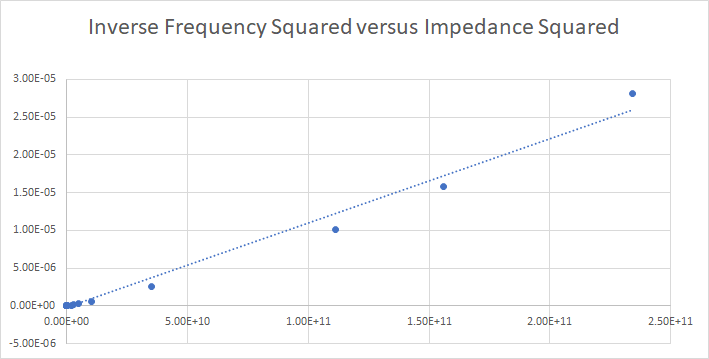
\includegraphics[width=0.85\textwidth]{boxalinear}
\end{figure}

Using the fact that slope is equal to ${C^2}$ and intercept is $\frac{1}{R^{2}}$, the capacitance turns out to be $2.0\times 10^{-7}F$ and the resistance $8.0\times 10^{32}\Omega$. This is inconsistent with our hypothesis of the resistor. Due to this reason, a new hypothesis will be formed where the resistor will be thrown out. The new hypothesis, supported by the experimental data, is the following:
\begin{figure}[h]
\centering
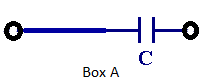
\includegraphics[width=0.5\textwidth]{boxaconfig2}
\end{figure}
\clearpage
\subsection{Box E}
The DC resistance of this box was found to be too large for the multimeter to detect. Therefore, a capacitor in series exists between the two terminals of the box, with no parallel configuration. The data obtained for this box is the following:
\begin{figure}[h]
\centering
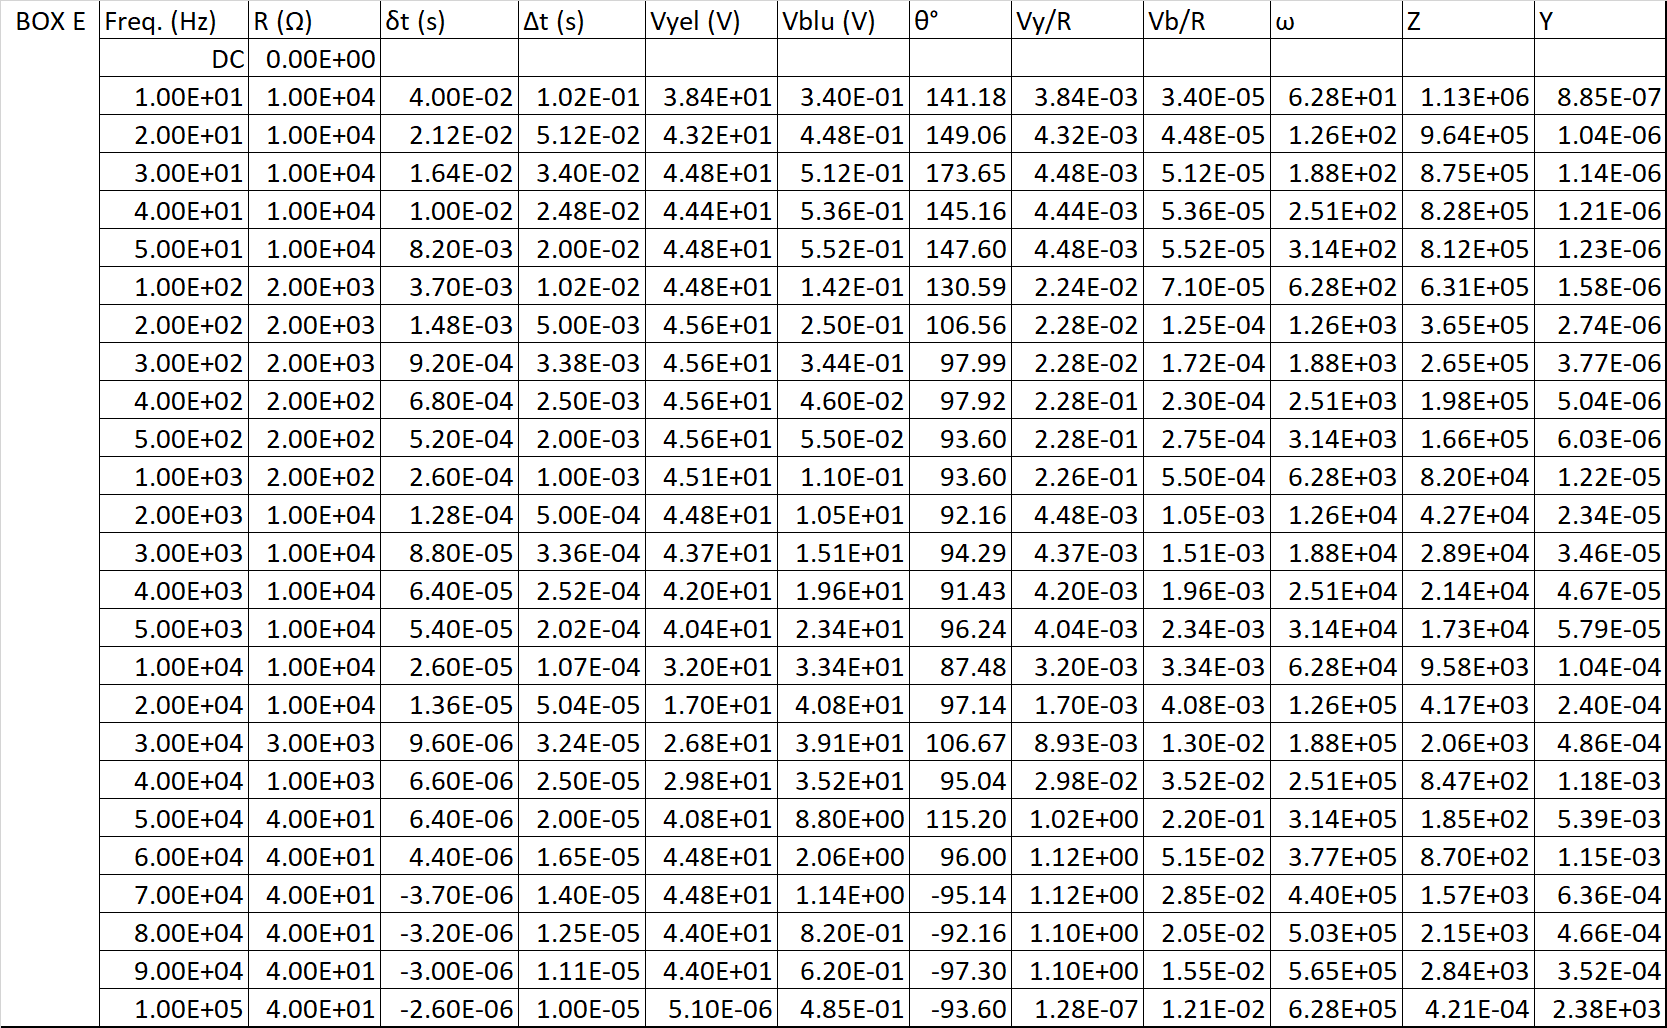
\includegraphics[width=1.0\textwidth]{boxe}
\end{figure}

The same procedure was used to plot the graph of impedance versus angular frequency. The resulting plot is the following:
\begin{figure}[h]
\centering
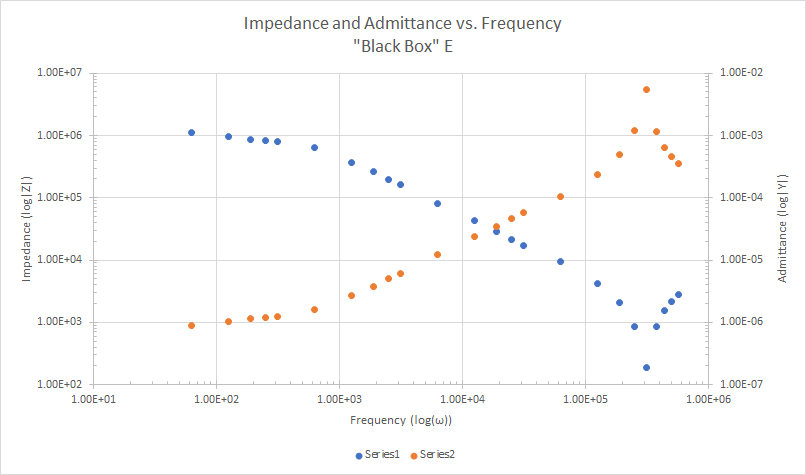
\includegraphics[width=0.71\textwidth]{boxeplot}
\caption{Graph of impedance vs. log of frequency for Box D. The admittance $|Y|=\frac{1}{|Z|}$ was plotted on top for visualization purposes and qualitative understanding.}
\end{figure}

As it can be seen from the graph, there exist resonance. This behavior is indicative of the existence of an inductor, in series with the capacitor. In addition, there is a decrease in impedance with frequency, until a certain frequency where impedance begins to raise. This corroborates the existence of a capacitor. Inductors contribute less at lower frequencies, allowing current to pass through. On the contrary, high frequencies annihilates the purpose of the capacitor as it does not have much time to charge up and increase impedance. 

Focuising on high frequencies where the inductor rules, we can obtain a linear regression with the purpose of finding the resistance and inductance of the components, the following equation will be used:
\begin{equation}
Z=L^2w^2+R^2
\end{equation}

By plotting $Z^2$ vs. $w^2$, we are able to obtain a linear regression with slope equal to the inductance of the inductor and intercept equal to $R^2$. The resulting plot is the following:
\begin{figure}[h]
\centering
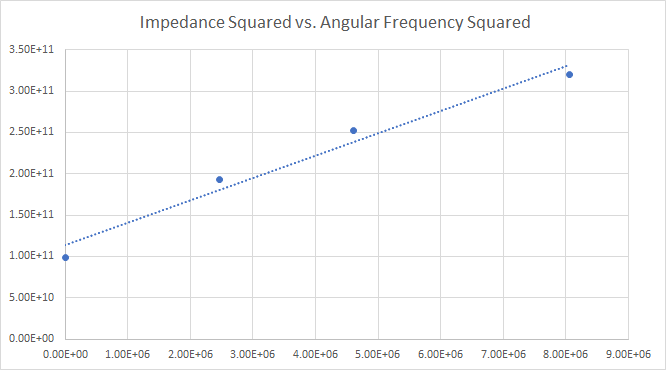
\includegraphics[width=0.85\textwidth]{boxelinear}
\end{figure}

Using the previous properties, the inductance was measured to be $6.8\times 10^{-3}H$. Using the equation $C=\frac{1}{w^2L}$, the capacitance was found the be $1.2\times 10^{-9}F$. In addition, the intercept allowed the calculation for the resistance of the box, turning out to be $102.4\Omega$. The existence of a resistor is forced by the fact that there is an inductor present in the box. Therefore, our hypothesis for the components of Box E is a simple RLC circuit in series, as shown below:
\begin{figure}[h]
\centering
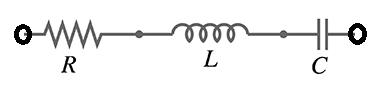
\includegraphics[width=0.5\textwidth]{boxeconfig}
\end{figure}

Where the corresponding values are:
\begin{figure}[h]
\[R=102.4\Omega\]
\[L=6.8\times 10^{-3}H\]
\[C=1.2\times 10^{-9}F\]
\end{figure}
\clearpage

\subsection{Nonlinear Elements}

Using the same circuit as for the previous experiments, the diode was placed in the circuit in place of the box Z. Negative voltage resulted in no current through the diode. This can be seen from the signature of the component using the XY mode on the oscilloscope. The following signature was observed:
\begin{figure}[h]
\centering
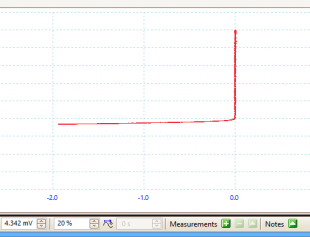
\includegraphics[width=0.35\textwidth]{signature}
\end{figure}

This function plots a trace of the components behavior to flow of charge and potential difference. The current generates a vertical trace deflection on the display, while the voltage across the diode generates a horizontal trace deflection. This results in a well-defined trace on the display that provides an analog signature for the component. The existence of a right-angled line is consistent with the behavior of the diode, as there is no current in the opposite direction.

Lastly, we can notice the existence of a threshold voltage that allow current to flow. For different frequencies, the threshold voltage was plotted. The resulting graph is the following:
\begin{figure}[h]
\centering
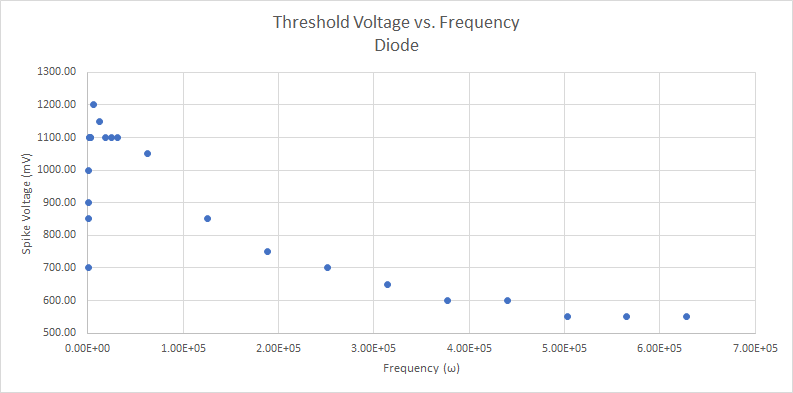
\includegraphics[width=0.75\textwidth]{spike}
\caption{Spike voltage as a function of frequency. The higher the frequency, the lower the threshold voltage. This might be due to the residual voltage left by the rapid frequencies.}
\end{figure}
\clearpage
\section{Conclusion}
\subsection{Output Impedance}
Using the multimeter, the  voltage of the battery was found to be $8.37V$. To verify this, a load resistor was placed in series with the battery. Various values of resistance were recorded and the corresponding voltage was reported. Using Ohm's Law the current was calculated. Using the linear regression $V=V_0-IR_0$, the internal resistance was found to be $839.2\Omega$, and the output voltage $8.59$. The voltage inconsistency with the multimeter might be caused by an irregular battery or to heat caused by data taking. For a future experiment, it might be a good idea to let the circuit cool down before doing successive measurements.
\subsection{Unknown Linear Black Boxes}
\subsubsection{Box D}
Box D was hypothesized to be a resistor and a capacitor in series. The experimental data strongly agreed with the hypothesis. The resistance was found to be $R=1329.7\Omega$, while the capacitance was $C=3.3\times 10^{-7}$.
\subsubsection{Box A}
Box A was hypothesized to be a single capacitor in series with the two terminals of the box. The presence of an inductor and a resistor in any configuration was ruled out by the experimental data. The capacitance of this component was found to be $C=2.0\times 10^{-7}F$. 
\subsubsection{Box E}
The components of box E were guessed to be an RLC circuit in series. The resistor had a value of $R=102.4\Omega$, the inductor $L=6.8\times 10^{-3}H$ and the capacitor $C=1.2\times 10^{-9}$.
\subsubsection{Nonlinear Elements}
The diode was observed to flow current in only one direction. In addition, the threshold voltage was found to decrease as frequency increases.
\clearpage
\section{References}
\begin{itemize}
\item Physics 133 2018 Lab Manual at University of California Santa Cruz
\end{itemize}







  
  \end{document}